% \documentclass[12pt, twoside]{article}
\usepackage[letterpaper, margin=1in, headsep=0.2in]{geometry}
\setlength{\headheight}{0.6in}
%\usepackage[english]{babel}
\usepackage[utf8]{inputenc}
\usepackage{microtype}
\usepackage{amsmath}
\usepackage{amssymb}
%\usepackage{amsfonts}
\usepackage[nomessages]{fp} %\FPeval{\var-name}{2*sin(pi/6)}
\usepackage{siunitx} %units in math. eg 20\milli\meter
\usepackage{yhmath} % for arcs, overparenth command
\usepackage{tikz} %graphics
\usetikzlibrary{quotes, angles, arrows, arrows.meta}
\usepackage{graphicx} %consider setting \graphicspath{{images/}}
\usepackage{parskip} %no paragraph indent
\usepackage{enumitem}
\usepackage{multicol}
\usepackage{venndiagram}

\usepackage{fancyhdr}
\pagestyle{fancy}
\fancyhf{}
\renewcommand{\headrulewidth}{0pt} % disable the underline of the header
\raggedbottom
\hfuzz=2mm %suppresses overfull box warnings

\usepackage{hyperref}

\fancyhead[LE]{\thepage}
\fancyhead[RO]{\thepage \\ Name: \hspace{4cm} \,\\}
\fancyhead[LO]{BECA / Dr. Huson / Geometry\\*  Unit 3: Parallel lines and transversals\\* 17 October 2022}

\begin{document}

\subsubsection*{3.1 Homework: Mixed review}
\begin{enumerate}
\item Two lines intersect with vertical angles m$\angle 1=2x+20$ and m$\angle 3=3x-5$. Find m$\angle 2$.
  \begin{flushleft}
  \begin{tikzpicture}[scale=0.8, rotate=30]
    \draw[<->, thick] (0,-1.5)--(10,1.5);
    \draw[<->, thick] (2,3.5)--(7,-3.5);
    \node at (1.5,1.3){m$\angle 1=2x+20$};
    \node at (7,-1){m$\angle 3=3x-5$};
    \node at (5,1){2};
    \node at (4,-1){4};
  \end{tikzpicture}
  \end{flushleft}

\item Write the appropriate name for the type of angle depending on its measure in degrees. (acute, right, obtuse, or straight)
    \begin{enumerate}
      \item m$\angle = 90$ : \rule{4cm}{0.15mm} \bigskip
      \item $90 < \text{m}\angle < 180$ : \rule{4cm}{0.15mm} \bigskip
      \item $0< \text{m}\angle < 90$ : \rule{4cm}{0.15mm} \bigskip
      \item m$\angle = 180$ : \rule{4cm}{0.15mm} \bigskip
    \end{enumerate}

\item Identify the true statement(s) given $\angle AOB = 2x$ and $\angle BOC = 5x+20$.
 \begin{multicols}{2}
    \begin{enumerate}
      \item $\angle AOB \cong \angle BOC$\\
      $2x = (5x+20)$
      \item $\angle AOB$, $\angle BOC$ are complementary\\
      $2x + (5x+20)=90^\circ$
      \item $\angle AOB$ and $\angle BOC$ are a linear pair\\
      $2x + (5x+20)=180^\circ$
  \end{enumerate}
  \begin{center}
    \begin{tikzpicture}[scale=0.7, rotate=20]
      \draw[<->, thick] (-45:5)--(0,0)--(135:5);
      \draw[<->, thick] (-5,0)--(5,0);
      \draw[->, thick] (0,0)--(0,4);
      \draw (0,0)++(0.3,0)--++(0,0.3)--+(-0.3,0);
      \draw[fill] (135:3) circle [radius=0.05] node[below left]{$B$};
      \draw[fill] (-4,0) circle [radius=0.05] node[below]{$A$}; 
      \draw[fill] (0,0) circle [radius=0.05] node[below]{$O$};
      \draw[fill] (0,3) circle [radius=0.05] node[left]{$C$};
      \draw[fill] (4,0) circle [radius=0.05] node[below]{$D$};
      \draw[fill] (-45:3) circle [radius=0.05] node[above]{$E$};
      \end{tikzpicture}
  \end{center}
\end{multicols}
Copy the correct equation and solve for $x$. Check your answer. \vspace{2cm}

\newpage
  
\item As shown below, two lines intersect making four angles: $\angle 1$, $\angle 2$, $\angle 3$, and $\angle 4$.
\begin{multicols}{2}  
  \begin{enumerate}
    \item Name a pair of vertical angles. \vspace{1.cm}
    \item Given m$\angle 4 = 70^\circ$, write down m$\angle 2$. \vspace{1.cm}
    \item Find m$\angle 1$. \vspace{2cm}
  \end{enumerate}
  \begin{tikzpicture}[scale=0.7, rotate=-20]
  \draw[<->, thick] (0,-1.5)--(10,1.5);
  \draw[<->, thick] (2.5,2)--(7,-3);
  \node at (3,.4){4};
  \node at (6,-.6){2};
  \node at (5,1){1};
  \node at (4,-1){3};
\end{tikzpicture}
\end{multicols} \vspace{1cm}

\item As shown below, two lines intersect making four angles: $\angle 1$, $\angle 2$, $\angle 3$, and $\angle 4$. Given that m$\angle 1= x+32$ and m$\angle 3=2x-8$, find m$\angle 1$.
  \begin{flushright}
    \begin{tikzpicture}[scale=1, rotate=0]
      \draw[<->, thick] (1,-1)--(8,1);
      \draw[<->, thick] (3,2)--(6,-2);
      \node at (2,.3){m$\angle 1= x+32$};
      \node at (6.5,-.3){m$\angle 3=2x-8$};
      \node at (5,1){2};
      \node at (4,-1){4};
    \end{tikzpicture}
    \end{flushright} \vspace{2cm}

\item An angle bisector is shown below, with $\overrightarrow{PR}$ bisecting $\angle QPS$. Given m$\angle QPR = 3x-2$ and m$\angle RPS = 2x+23$, find m$\angle QPS$.
  \begin{flushright}
  \begin{tikzpicture}[scale=0.6, rotate=-60]
    \draw[<->, thick] (230:5)node[left]{$Q$} 
    --(0,0)node[below]{$P$}
    --(110:6)node[below right]{$S$}--(110:7);
    \draw[->, thick] (0,0)--(170:7)node[right]{$R$};
  \end{tikzpicture}
  \end{flushright} \vspace{1cm}


\end{enumerate}
\end{document}